
\hypertarget{cosets-and-lagrange}{%
\section{Cosets and Lagrange}\label{cosets-and-lagrange}}

\begin{definition}
Let \(H \leq G\) and \(g \in G\).
The \emph{left coset \(gH\)} is defined to be \(\{ gh : h \in H \}\).
Similarly the \emph{right coset} \(Hg = \{ hg : h \in H \}\)
\end{definition}

\begin{example}
\begin{align*}
    S_3 &= \{ e, \begin{pmatrix}1 & 2 & 3\end{pmatrix}, \begin{pmatrix}1 & 3 & 2\end{pmatrix}, \begin{pmatrix}1 & 2\end{pmatrix}, \begin{pmatrix}1 & 3\end{pmatrix}, \begin{pmatrix}2 & 3\end{pmatrix} \} \\
    H &= \{ \text{id}, \begin{pmatrix}1 & 2 & 3\end{pmatrix}, \begin{pmatrix}1 & 3 & 2\end{pmatrix} \} = A_3 \\
    \begin{pmatrix}1 & 2\end{pmatrix}H &= \left\{ \begin{pmatrix}1 & 2\end{pmatrix}, \begin{pmatrix}1 & 2\end{pmatrix}\begin{pmatrix}1 & 2 & 3\end{pmatrix}, \begin{pmatrix}1 & 2\end{pmatrix}\begin{pmatrix}1 & 3 & 2\end{pmatrix} \right\} \\
    &= \left\{ \begin{pmatrix}1 & 2\end{pmatrix}, \begin{pmatrix}2 & 3\end{pmatrix}, \begin{pmatrix}1 & 3\end{pmatrix} \right\} \\
    \begin{pmatrix}1 & 2 & 3\end{pmatrix}H &= H \ (\text{since H is a subgroup})
\end{align*}
Note, \(H \dot{\cup} \begin{pmatrix}1 & 2\end{pmatrix}H = S_3\)
\end{example}

\begin{lemma}
\protect\hypertarget{lem:nine}{}\label{lem:nine}Let \(H \leq G\) and \(g \in G\).
Then there is a bijection between \(H\) and \(gH\).
In particular if \(H\) is finite then \(|H| = |gH|\).
\end{lemma}

\begin{proof}
Define \(\theta_g : H\)
\begin{align*}
    \theta_g : H &\to gH \\
    h &\mapsto gh.
\end{align*}
We show \(\theta_g\) is a bijection.

Surjectivity: if \(gh \in gH\) then \(\theta_g(h) = gh\).

Injectivity: \begin{align*}
    \theta_g(h_1) &= \theta_g(h_2) \\
    g h_1 &= g h_2 \\
    \implies h_1 &= h_2 \ (\text{cancellation law})
\end{align*}
\end{proof}

\begin{lemma}
\protect\hypertarget{lem:ten}{}\label{lem:ten}

The left cosets of \(H\) in \(G\) form a partition of \(G\) i.e.

\begin{enumerate}
\def\labelenumi{\roman{enumi}.}
\item
  each \(g \in G\) lies in some left coset of \(H\) in G.
\item
  if \(aH \cup bH \neq \emptyset\) (for some \(a, b \in G\)) \(\implies aH = bH\).
\end{enumerate}

\end{lemma}

\begin{figure}

{\centering 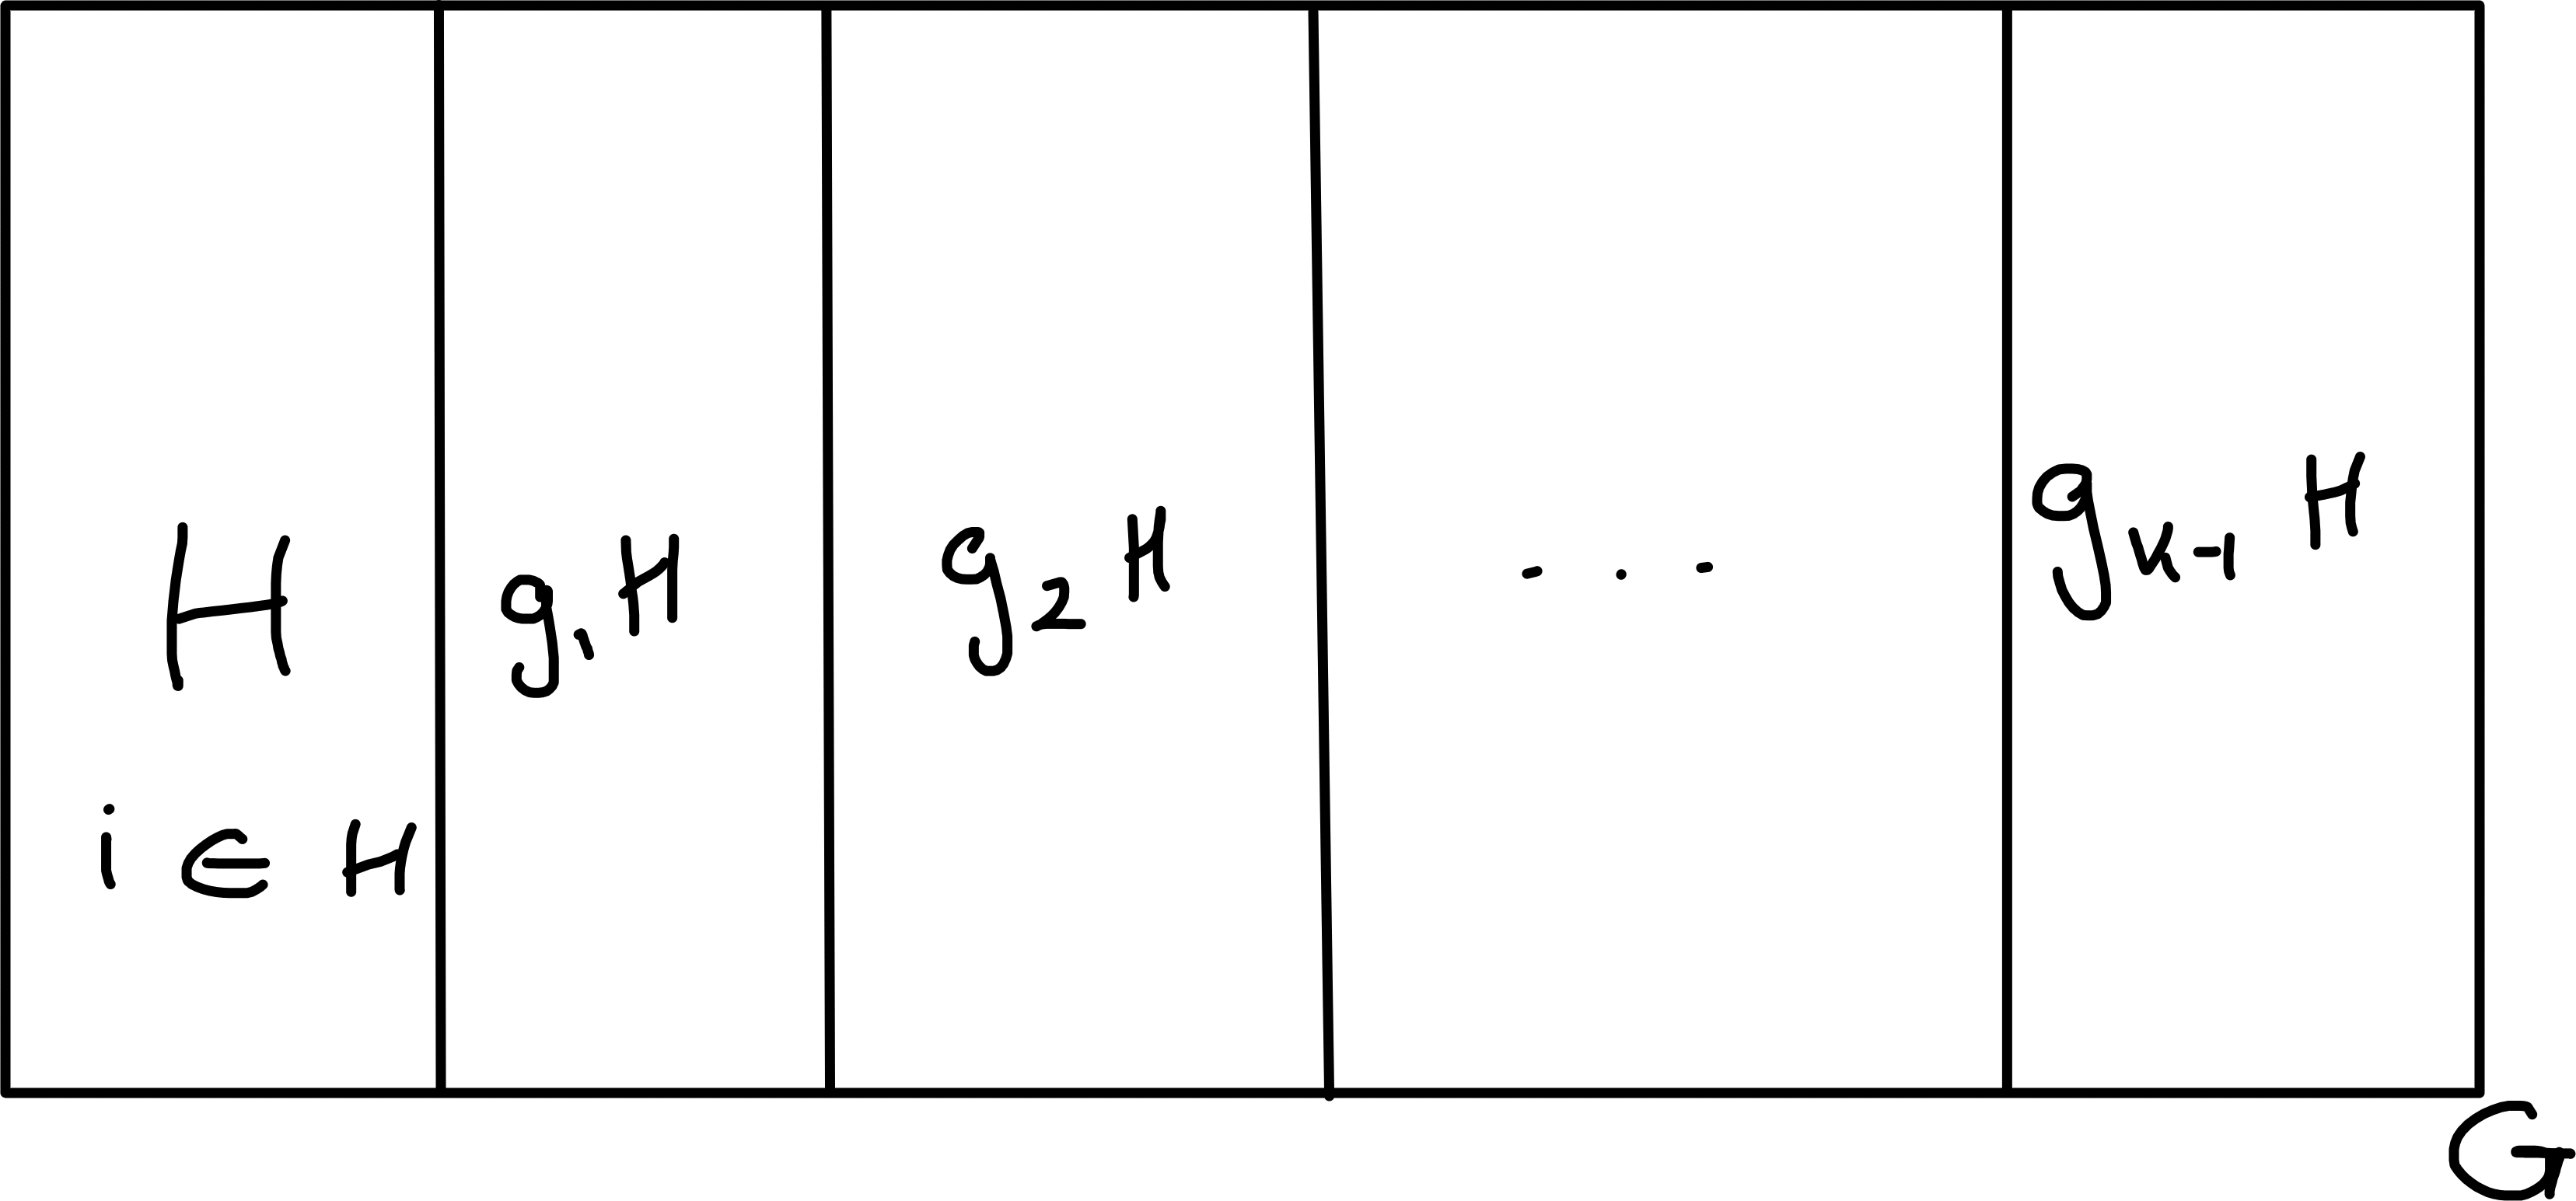
\includegraphics{figures/03-cosets} 

}

\end{figure}

\begin{proof}
~

\begin{enumerate}
\def\labelenumi{\roman{enumi}.}
\item
  \(g \in gH\) as \(e \in H\)
\item
  Suppose \(c \in aH \cup bH\).\\
  Claim: \(aH = cH = bH\).
\end{enumerate}

Now \(c \in aH\) so \(c = ak\) for some \(k \in H\).
\begin{align*}
    \implies cH &= \{ c h : h \in H \} \\
    &= \{ a k h : h \in H \} \subseteq aH.
\end{align*}

Similarly, \(a = c k^{-1} \in cH\)
\begin{align*}
    \implies aH \subseteq cH.
\end{align*}
So \(aH = cH\).\\
Similarly \(cH = bH\)
\end{proof}

\begin{example}
\(S_n = \underbrace{A_n}_\text{even elements} \dot{\cup} \underbrace{\begin{pmatrix}1 & 2\end{pmatrix} A_n}_\text{odd elements}\)
\end{example}

\begin{lemma}
\protect\hypertarget{lem:eleven}{}\label{lem:eleven}Let \(H \leq G\), \(a, b \in G\).
Then \(aH = bH \iff a^{-1} b \in H\).
\end{lemma}

\begin{proof}
\((\implies)\):
\begin{align*}
    b &\in bH = aH \\
    \implies b &= ah \text{ for some } h \in H \\
    \implies a^{-1} b &= h \in H
\end{align*}

\((\Longleftarrow)\):
\begin{align*}
    \text{Suppose } a^{-1}b &= k \in H \\
    \implies b &= ak \in aH \\
    \text{also } b &\in bH. \\
    \implies aH &= bH
\end{align*} by Lemma \ref{lem:ten}
\end{proof}

\begin{theorem}[Lagrange's Theorem]
\protect\hypertarget{thm:three}{}\label{thm:three}Let \(H\) be a subgroup of the finite group \(G\).
Then the order of \(H\) divides the order of \(G\) (i.e.~\(|H| \bigg| |G|\)).
\end{theorem}

\begin{proof}
By Lemma \ref{lem:ten} \(G\) is partitioned into distinct cosets of \(H\), say \(G = g_1 H \dot{\cup} g_2 H \dot{\cup} \ldots \dot{\cup} g_k H\) (say \(g_1 = e\)).\\
By Lemma \ref{lem:nine}
\begin{align*}
    |g_i H| &= |H| \hspace{.5cm} 1 \leq i \leq k \\
    \implies |G| &= |H|k
\end{align*}
\end{proof}

\footnote{You would need to prove these lemma's in an exam q.}

\begin{definition}
\protect\hypertarget{def:fourteen}{}\label{def:fourteen}Let \(H \leq G\).
The \emph{index} of \(H\) in \(G\) is the number of left cosets of \(H\) in \(G\), denoted \(|G : H|\).
\end{definition}

\begin{remark}

~

\begin{enumerate}
\def\labelenumi{\roman{enumi}.}
\item
  If \(G\) is finite, \(|G : H| = \frac{|G|}{|H|}\).
  But we can have \(|G : H|\) finite, even if \(G\) and \(H\) are infinite, e.g.~\(\mathbb{Z}\) and \(n\mathbb{Z}\) where \(|G : H| = n\).
\item
  We write \((G : H)\) for the set of left cosets of \(H\) in \(G\).
\end{enumerate}

\end{remark}

\begin{corollary}[Lagrange's Corollary]
\protect\hypertarget{cor:two}{}\label{cor:two}\(G\) is a finite group, \(g \in G\).
Then \(o(g) \bigg| |G|\).
In particular, \(g^{|G|} = e\).
\end{corollary}

\begin{proof}
\begin{align*}
    \text{Note } \left\langle g\right\rangle &= \{ e, g, \ldots, g^{n-1} \} \text{ where } o(g) = n. \\
    \text{Then } o(g) &= | \left\langle g\right\rangle | \bigg| |G| \text{ by Lagrange} \\
    \implies g^{|G|} &= e \text{ by Lemma }
\end{align*} \ref{lem:five}
\end{proof}

\begin{corollary}
\protect\hypertarget{cor:three}{}\label{cor:three}If \(|G| = p\) for some prime \(p\), then \(G\) is cyclic.
\end{corollary}

\begin{proof}
Let \(e \neq g \in G\).
Then \(\{ e \} \neq \langle g \rangle \leq G\).
By Lagrange
\begin{align*}
    1 &\neq | \langle g \rangle | \;\bigg|\; |G| = p \\
    \implies | \langle g \rangle | &= p = |G| \\
    \implies \langle g \rangle &= G
\end{align*}
i.e.~\(G\) cyclic.
\end{proof}

Euler's totient function.\\
Let \(n \in \mathbb{N}\) and \(\phi(n) = \left| \left\{ a \leq a \leq n : \operatorname{hcf}(a, n) = 1 \right\} \right|\) so \(\phi(12) = \left| \left\{ 1, 5, 7, 11 \right\} \right| = 4\).

\begin{theorem}[Fermat-Euler Theorem]
\protect\hypertarget{thm:four}{}\label{thm:four}Let \(n \in \mathbb{N},\ a \in \mathbb{Z}\) and \(\operatorname{hcf}(a, n) = 1\).\\
Then \(a^{\phi(n)} \equiv 1 \pmod n\).
\end{theorem}

We can prove this by using Lagrange, but first we need to set it up.\\
Let \(n \in \mathbb{N}\),
\begin{align*}
    R_n &= \{ 0, 1, \ldots, n-1 \} \\
    R_n^* &= \{ a \in R_n : \operatorname{hcf}(a, n) = 1 \}
\end{align*}
Define \(\times_n\) to be multiplication mod \(n\).\\
Claim: \((R_n^*, \times_n)\) is a group.
Notation, \(n \in \mathbb{Z}\) then \(\bar{u} \in R_n\) such that \(u \equiv \bar{u} \pmod n\).

Closure:
\begin{align*}
    \operatorname{hcf}(a, n) &= 1 = \operatorname{hcf}(b, n)
    \implies \operatorname{hcf}(ab, n) = 1 \\
    \implies \operatorname{hcf}(\bar{ab}, n) = 1 \\
\end{align*}

Identity = 1

Associativity is fine.

Inverses: Let \(a \in R_n^*\), \(\operatorname{hcf}(a, n) = 1\)
\begin{align*}
    \implies \exists \; u, v \in \mathbb{Z} s.t. a u + v n = 1 \text{ (Bezout's Theorem)} \\
    \implies au \equiv 1 \pmod n
\end{align*}
Then \(\bar{u} \in R_n^*\) is \(a^{-1}\)

\begin{proof}
Note \(|R_n^*| = \phi(n)\).
\begin{align*}
    a \equiv \bar{a} \pmod n,\ \bar{a} \in R_n^*
\end{align*}
By Corollary \ref{cor:two}
\begin{align*}
    \bar{a}^{\phi(n)} &= \bar{a}^{|R_n^*|} = 1 \in R_n^* \\
    \implies a^{\phi(n)} &\equiv 1 \pmod n
\end{align*}
\end{proof}
